Co vše provádí operační systém:
\begin{itemize}
\item Organizuje přístup a \textbf{využívání zdrojů počítače }(čas procesoru, přístup k datům na discích, přístup do paměti).
\item Fyzicky zajišťuje \textbf{vstup} a \textbf{výstup} dat podle požadavků ostatních programů.
\item\textbf{ Komunikuje s uživatelem} a na základě jeho pokynů vykonává požadované akce.
\item \textbf{Reaguje na chybové stavy} programů a mylné požadavky uživatelů tak, aby tyto chyby nezpůsobily zásadní destrukci systému nebo poškození dat.
\item \textbf{Spravuje komunikaci s periferiemi}. Definuje nastavení klávesnice, citlivost myši a dalších zařízení.
\item Eviduje využívání systémových zdrojů apod.
\end{itemize}

\subsection{Struktura OS}
Operační systém je zpravidla tvořen tzv. \textbf{jádrem} (kernel), \textbf{ovladači I/O zařízení} (driver), \textbf{příkazovým procesorem} (shell) a \textbf{podpůrnými systémovými programy}.
\begin{itemize}
	\item \textbf{Jádro} -- po \textbf{zavedení} do paměti \textbf{řídí} činnost počítače, poskytuje procesům služby a řeší správu prostředků a správu procesů.
	\item \textbf{Ovladač} -- zvláštní (pod)program pro \textbf{ovládání konkrétního zařízení} standardním způsobem. Použití strategie s ovladači umožňuje snadnou konfigurovatelnost technického vybavení.
	\item \textbf{Příkazový procesor} -- program, který \textbf{umožňuje} uživatelům \textbf{zadávat příkazy} ve speciálním, obvykle jednoduchém jazyce.
	\item \textbf{Podpůrné programy} -- do této kategorie jsou mnohdy zahrnovány i překladače (jazyk C v OS UNIX) a sestavující programy. Stojí na stejném místě jako aplikační programy.
\end{itemize}

\subsection{Jádro}
Jádro se zpravidla dělí na dvě podstatné části:
\begin{enumerate}
	\item \textbf{Správa procesů} -- řeší problematiku aktivování a deaktivování procesů podle jejich priority resp. požadavků na prostředky (prakticky není u jednoduchých OS)
	\item \textbf{Správa prostředků} -- zajištuje činnost I/O zařízení, přiděluje paměť, případně procesory. Velmi důležitou částí správy prostředků je \textbf{správa souborů} -- způsob ukládání souborů a přístupu k nim. Moderní OS zajištují jednotný pohled na soubory a zařízení. Zařízení jsou považovány za soubory se speciálním jménem.
\end{enumerate}

\subsection{Generické komponenty OS} % https://publi.cz/books/11/04.html
\begin{minipage}[t]{0.6\textwidth}
	\begin{itemize}
		\item správa \textbf{procesorů},
		\item správa \textbf{procesů} (proces – činnost řízená programem),
		\item správa vnitřní \textbf{(hlavní) paměti},
		\item správa \textbf{souborů},
		\item správa \textbf{I/O} systému,
		\item správa vnější \textbf{(sekundární) paměti},
		\item \textbf{networking}, distribuované systémy,
		\item systém ochran,
		\item \textbf{interpret příkazů}.
	\end{itemize}
\end{minipage}
\begin{minipage}[t]{0.38\textwidth}
	\vspace{-10mm}
	\begin{figure}[H]
		\centering
		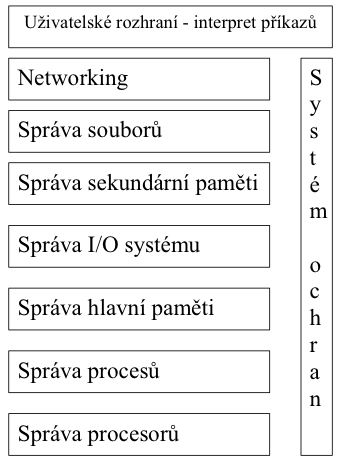
\includegraphics[width=0.9\textwidth]{assets/3_gen_komp_os}
	\end{figure}
\end{minipage}

\subsubsection{Správa procesorů/procesů}
Pojem \textbf{proces} (task) je nějaká činnost řízená programem. Proces potřebuje pro svou realizaci jisté zdroje (dobu procesoru, paměť, I/O zařízení, atd.). OS je z hlediska \textbf{správy procesů} zodpovědný za:
\begin{itemize}
	\item \textbf{sleduje prostředek} (procesor a stav procesů),
	\item \textbf{vytváření} a \textbf{rušení} procesů,
	\item \textbf{potlačení} a \textbf{obnovení} procesů,
	\item poskytnutí mechanismů pro \textbf{synchronizaci} procesů a pro \textbf{komunikaci} mezi procesy,
	\item požaduje vrácení prostředku (procesoru).
\end{itemize}
OS je z hlediska \textbf{správy procesorů} zodpovědný za výběr procesu běžícího na volném procesoru. Dále podle typu OS zde patří i \textbf{plánování vláken}.

\subsubsection{Správa (hlavní, operační) paměti}
Jedná se o \textbf{úložiště} připravených tj. \textbf{rychle dostupných dat} sdílených procesorem a I/O zařízeními. Hlavní paměť je pole samostatně adresovatelných slov nebo bytů, zpravidla energeticky závislá. OS je z hlediska správy \textbf{(hlavní) paměti} odpovědný za:
\begin{itemize}
	\item vedení přehledů \textbf{kdo} a \textbf{kterou část paměti v daném okamžiku využívá},
	\item ve spolupráci se správou procesů \textbf{rozhoduje} o tom, kterému procesu, kolik, kde a kdy má přidělit operační paměť,
	\item \textbf{přidělování} a \textbf{uvolňování} paměti dle potřeby,
	\item řízení virtuální paměti.
\end{itemize}

\subsubsection{Správa I/O systému}
Správce periferních (I/O systému) má tyto funkce:
\begin{itemize}
	\item sleduje \textbf{stav prostředků }(periferních zařízení, jejich řídících jednotek),
	\item \textbf{rozhoduje} o\textbf{ efektivním způsobu přidělování prostředku} -- periferního zařízení,
	\item \textbf{přiřazuje} prostředek (periferní zařízení) a zahajuje I/O operaci,
	\item požaduje \textbf{navrácení} prostředku.
\end{itemize}
Z hlediska funkce OS lze správce I/O systému chápat jako:
\begin{itemize}
	\item úložiště \textbf{vyrovnávacích pamětí},
	\item univerzální rozhraní ovladače I/O zařízení,
	\item \textbf{ovladače} jednotlivých hardwarových I/O zařízení.
\end{itemize}

\subsubsection{Správa vnější paměti}
Do správy I/O systému patří i \textbf{správa vnější (sekundární) paměti}. Počítačový systém musí poskytnout pro zálohování hlavní paměti sekundární paměť (HDD, SSD). OS je z hlediska správny vnější (sekundární) paměti odpovědný za:
\begin{itemize}
	\item správu \textbf{volné} paměti,
	\item \textbf{přidělování} paměti,
	\item plánování činnosti disku.
\end{itemize}

\subsubsection{Správa souborů}
Správce souborů má tyto funkce:
\begin{itemize}
	\item sleduje prostředek (soubor), jeho umístění, užití, stav atd.,
	\item rozhoduje, komu budou prostředky \textbf{přiděleny}, realizuje požadavky na \textbf{ochranu informací uložených} v souborech a realizuje operace přístupu k souborům,
	\item \textbf{přiděluje} prostředek, tj. otevírá soubor,
	\item \textbf{uvolňuje} prostředek, tj. uzavírá soubor.
\end{itemize}
Pod pojmem soubor chápeme jak programy, tak data. OS je z hlediska správy souborů odpovědný za:
\begin{itemize}
	\item vytváření a rušení souborů,
	\item vytváření a rušení adresářů (katalogů, složek),
	\item podporu primitivních \textbf{operací} pro manipulaci se soubory a adresáři,
	\item archivování souborů na energeticky nezávislá média.
\end{itemize}
\subsubsection{Networking, distribuované systémy}
Distribuovaný systém je \textbf{kolekce procesorů}, které \textbf{nesdílejí} ani \textbf{fyzickou paměť} ani \textbf{hodiny}, synchronizující činnost procesoru. Každý procesor má svoji \textbf{lokální paměť} a \textbf{lokální hodiny}. Procesory distribuovaného systému jsou \textbf{propojeny} komunikační sítí. Komunikace jsou řízeny protokoly. Distribuovaný systém uživateli zprostředkovává přístup k různým zdrojům systému.

\subsubsection{Systém ochran}
Jsou to mechanismy pro \textbf{řízení přístupu} k \textbf{systémovým} a \textbf{uživatelským zdrojům}. Systém ochran musí:
\begin{itemize}
	\item \textbf{rozlišovat} mezi \textbf{autorizovaným} a \textbf{neautorizovaným} použitím,
	\item specifikovat problém vnucovaného řízení,
	\item poskytnout prostředky pro své prosazení.
\end{itemize}

\subsubsection{Uživatelské rozhraní - interpret příkazů}
Interpret příkazů je program, umožnující vykonávat příkazy pro:
\begin{itemize}
	\item \textbf{správu a vytváření procesů} -- služby OS poskytované interperetem příkazů slouží k \textbf{provedení programu}, tj. k schopnosti OS zavést program do hlavní paměti a spustit jeho běh,
	\item \textbf{ovládání I/O zařízení} -- uživatelský program \textbf{nesmí} provádět I/O operace \textbf{přímo}, OS musí poskytovat prostředky k provádění I/O operací,
	\item \textbf{správu sekundární paměti} -- manipulace se systémem souborů, schopnost číst, zapisovat, vytvářet a rušit soubory,
	\item správu hlavní paměti,
	\item zpřístupňování souborů,
	\item \textbf{ochranu} -- \textbf{detekci chyb v procesoru} a \textbf{paměti}, I/O zařízeních a v programech uživatelů pro zajištění správnosti výpočtu,
	\item \textbf{práci v síti} -- \textbf{výměna informací} mezi procesy realizována buďto v rámci jednoho počítače nebo mezi různými počítači pomocí sítě, tj. implementace sdílenou pamětí nebo předávání zpráv.
\end{itemize}
Uživatelská rozhraní jsou realizovaná \textbf{znakově} (command line) nebo \textbf{graficky}. Znakově orientovaným interpretům zadáváme příkazy pomocí klíčových slov, graficky orientovaným pomocí poklepání myši nebo dotykem na dotykové obrazovce na ikonu, pomocí dialogů apod.

\subsubsection{Vnitřní služby operačního systému}
Vnitřní služby OS \textbf{nejsou} určeny k tomu, aby \textbf{pomáhaly uživateli}, v prvé řadě slouží pro \textbf{zabezpečení efektivního provozu systému}, tj. slouží pro:
\begin{itemize}
	\item Přidělování prostředků (zdrojů) mezi více souběžně operujících uživatelů nebo úloh.
	\item Účtování a udržování přehledu o tom, kolik jakých zdrojů systému který uživatel používá. Cílem je účtování za služby a sběr statistik pro plánování.
	\item Ochranu tj. péči o to, aby veškerý přístup k systémovým zdrojům byl pod kontrolou.
\end{itemize}
Vnitřní služby OS jsou obecně \textbf{realizovány souborem systémových programů} vytvářejících určité systémové struktury tzv. virtuální stroje. Typickými službami jsou programy pro:
\begin{itemize}
	\item práci se soubory, editaci souborů, katalogizaci souborů, modifikaci souborů,
	\item získávání, definování a údržbu systémových informací,
	\item podporu jazykových prostředí,
	\item zavádění a provádění programů,
	\item komunikace a řízení aplikačních programů.
\end{itemize}

\subsection{Struktura OS podle jádra}
\begin{itemize}
	\item \textbf{Monolitická} jádra (monolithic kernel), \textbf{Mikrojádra} (microkernel), \textbf{Hybridní jádra}, \textbf{Nano jádra}.
\end{itemize}
\subsubsection{Monolitické jádro}
Monolitické jádro je druh jádra operačního systému, jehož \textbf{veškerý kód běží ve stejném (jaderném) paměťovém prostoru}, který se anglicky označuje jako \textbf{kernel space}. 

Tím se liší od tzv. mikrojádra, které většinu tradičních činností monolitického jádra, jako je třeba správa souborových systémů, implementuje v procesech, které běží v uživatelském paměťovém prostoru.
\begin{figure}[H]
	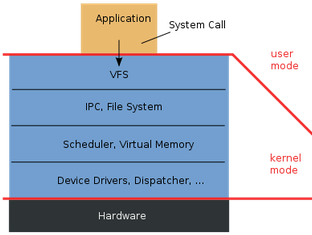
\includegraphics[width=0.5\textwidth,center]{assets/3_mon_os}
\end{figure}

\subsubsection*{Výhody}
\begin{itemize}
	\item[$+$] \textbf{dobrý výkon},
	\item[$+$] jednoduchost koncepce.
\end{itemize}
\subsubsection*{Nevýhody}
\begin{itemize}
	\item[$-$] \textbf{stabilita} -- jednotlivé části subsystémů sdílejí stejný paměťový prostor, může tak \textbf{chyba} v jednom subsystému zablokovat jiný, nebo dokonce \textbf{shodit celé jádro},
	\item[$-$] v případě větších jader OS jsou \textbf{těžko udržitelné},
	\item[$-$] mohou být obrovské (co se týče řádků kódu),
	\item[$-$] celková struktura je ve výsledku komplikovaná, neexistující hranice mezi moduly jádra.
\end{itemize}
\subsubsection*{Zástupci}
\begin{itemize}
\item Tradiční Unix kernely (včetně BSDs a Solaris), Linux, MS-DOS, Windows 9x, Mac OS (verze menší než 8.6).
\end{itemize}

\subsubsection{Mikrojádro}
Samotné jádro poskytuje jen \textbf{základní funkčnost nezbytnou pro vykonávání služeb}. Přístupem mikrojádra je definování jednoduché abstrakce hardware se soupravou primitivních funkcí nebo systémových volání implementujících minimální služby OS jako je \textbf{správa paměti} nebo \textbf{multitasking} (IPC). Ostatní služby včetně těch, které běžně poskytuje jádro, jsou \textbf{realizovány v uživatelském prostoru} (\textbf{userspace}).
\begin{figure}[H]
\centering
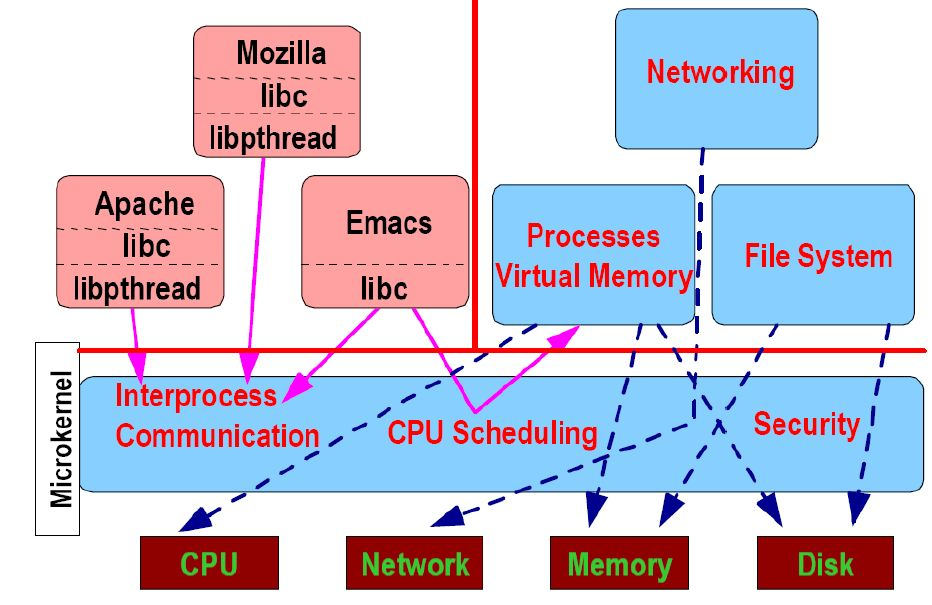
\includegraphics[width=0.6\textwidth]{assets/3_microkernel}
\end{figure}
\subsubsection*{Výhody}
\begin{itemize}
\item[$+$] jsou \textbf{stabilnější} a \textbf{bezpečnější} (každá služba je separátní proces) než monolitická jádra,
\item[$+$] procesy na uživatelské úrovni se nemusí zabývat hardwarem,
\item[$+$] jednoduché rozšíření na distribuovaný nebo multiprocesorový systém.
\end{itemize}
\subsubsection*{Nevýhody}
\begin{itemize}
\item[$-$] \textbf{pomalejší} než monolitická (\textbf{systémová volání}, zvyšují režii systému),
\item[$-$] nutné dodatečné \textbf{změny kontextu} (na rozdíl od monolitického (kde dojde při syscallu jen ke dvěma změnám mezi userspace a kernelspace) musí při dotazu na službu systému projít několika \textbf{změnami kontextu}).
\end{itemize}
\subsubsection*{Zástupci}
\begin{itemize}
\item AmigaOS, Amoeba, Mach, Minix, MorphOS, L4, QNX.
\end{itemize}

\subsubsection{Hybridní jádra}
Hybridní jádro se snaží \textbf{zkombinovat} rychlost a jednoduchost designu \textbf{monolitického} jádra s bezpečnostními výhodami \textbf{mikrojader}. 

Proto jsou hybridní jádra něco mezi monolitickým jádrem a mikrojádrem. To znamená že některé služby (jako souborový systém nebo implementace síťového protokolu) běží v jádře (\textbf{kernelspace}) ke zredukování režie proti mikrojádrům, ale jiné části monolitického jádra (ovladače zařízení) běží jako proces (\textbf{server}) v uživatelském prostoru (\textbf{userspace}).

\subsubsection*{Zástupci}
\begin{itemize}
\item NT kernel (used in Windows NT, 2000, XP, Vista and Windows 7), Darwin (Mac OS X's kernel), DragonFly BSD, BeOS, Plan 9.
\end{itemize}
\begin{figure}[H]
	\centering
	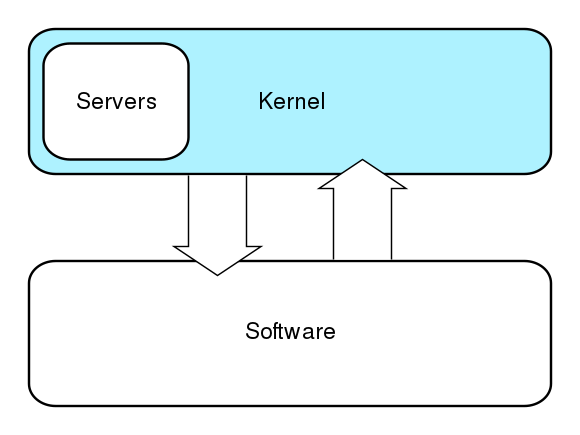
\includegraphics[width=0.4\textwidth]{assets/3_hybridkernel}
\end{figure}

\subsubsection{Nano jádra}
V nanojádru jsou \textbf{téměř všechny služby} – dokonce i ty nejzákladnější jako správce přerušení nebo časovač – řešeny ovladači zařízení. Tím má vlastní jádro\textbf{ ještě menší požadavky na paměť než mikrokernel}.

\subsection{Systémová volání}
Systémové volání (\textbf{syscall}) je v informatice mechanismus používaný aplikacemi k \textbf{volání funkcí operačního systému}, který se používá u jader systému monolitického typu. Najdeme je u všech unixových systémů. Systémy Microsoft Windows mají hybridní jádro a používají \textbf{meziprocesovou komunikaci} prostřednictvím Windows API, kde programátor nerozlišuje mezi knihovní funkcí a využíváním služeb operačního systému.

\begin{figure}[H]
\centering
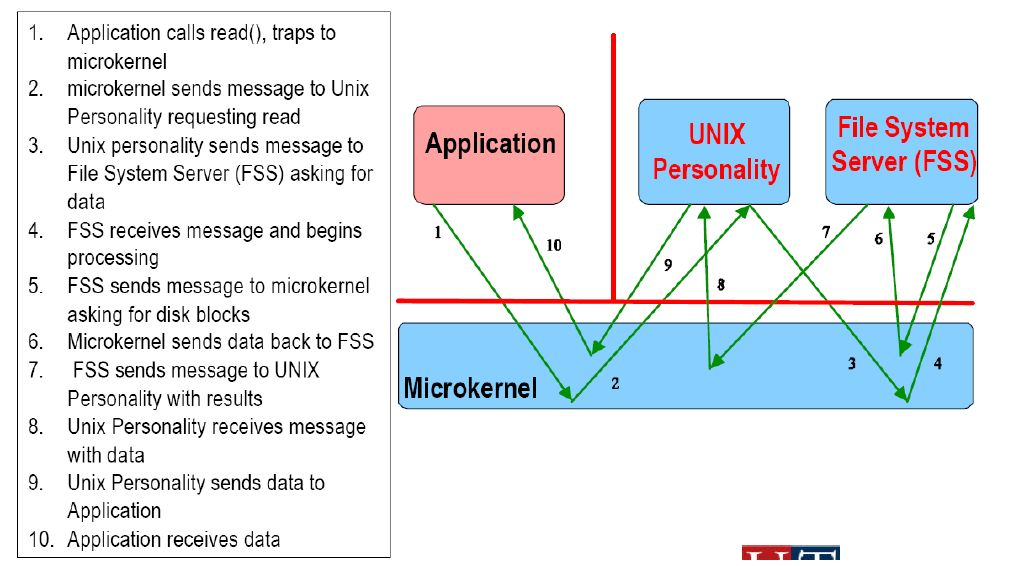
\includegraphics[width=1\textwidth]{assets/3_sys_call}
\end{figure}